\documentclass{UNESC}
\usepackage[T1]{fontenc}
\usepackage[utf8]{inputenc}%\usepackage[latin1]{inputenc}
\renewcommand{\rmdefault}{phv} % Arial
\renewcommand{\sfdefault}{phv} % Arial
\usepackage[brazilian]{babel}
\usepackage{graphicx}
\usepackage{hyperref}
\usepackage{quoting}
\usepackage[labelsep=none]{caption}
\DeclareCaptionLabelFormat{figuracomtraco}{#1~#2 -}
\captionsetup[figure]{labelformat=figuracomtraco, labelsep=space}
\captionsetup[table]{labelformat=simple, labelsep=space, textformat=simple}
\DeclareCaptionLabelFormat{tabelacomtraco}{#1~#2 -}
\captionsetup[table]{labelformat=tabelacomtraco}
\captionsetup{labelsep=none}
\captionsetup[table]{format=hang,justification=raggedright,
  singlelinecheck=false,labelsep=space,font=normalsize,
  labelfont=normalfont,textfont=normalfont,skip=6pt}
\usepackage{enumitem}
\usepackage{float}
\usepackage{comment}
\usepackage[hang,flushmargin]{footmisc}
\usepackage{array}
\usepackage{adjustbox}
\setlength{\emergencystretch}{3em}

\hypersetup{
  setpagesize  = false,
  colorlinks   = true,
  urlcolor     = blue,
  linkcolor    = black,
  citecolor    = black
}

\urlstyle{same}
\usepackage{setspace}

\usepackage[alf,recuo=0.0cm,abnt-emphasize=bf]{abntex2cite} 

\title{REGISTRO DIGITAL ANIMAL: DIGITALIZANDO A IDENTIFICAÇÃO E CONTROLE DE VACINAÇÃO DE ANIMAIS DE ESTIMAÇÃO}
\author
{
   Gabriel Goulart de Souza\footnote{Curso de Ciência da Computação, Universidade do Extremo Sul Catarinense (Unesc), Criciúma - Santa Catarina - Brasil. gabriel.gsouzza6@unesc.net},
   Diorgines Mattos Machado\footnote{Coorientador(a), Curso de Ciência da Computação, Universidade do Extremo Sul Catarinense (Unesc), Criciúma - Santa Catarina - Brasil. diorginesmattos@unesc.net},
   Allan Farias Favaro\footnote{Orientador(a), Curso de Ciência da Computação, Universidade do Extremo Sul Catarinense (Unesc), Criciúma - Santa Catarina - Brasil. allanfavaro@gmail.com}
}

\begin{document}

\onehalfspacing

\maketitle

\noindent
\textbf{Resumo:} A dispersão de dados de identificação, vacinação e documentos clínicos dificulta a organização do histórico de animais de estimação. Este trabalho teve como objetivo desenvolver e avaliar o funcionamento de uma aplicação multiplataforma para cadastrar, organizar e consultar esses registros. A aplicação Registro Digital Animal foi desenvolvida como aplicação web progressiva, com autenticação, sincronização e persistência no PostgreSQL. A avaliação reuniu 15 cenários funcionais de caixa-preta, dois retornos preservados do setor veterinário e uma coleta complementar com cinco envios de quatro contas. Nesta última, um envio repetido foi desconsiderado, resultando em quatro avaliações e 24 respostas a afirmações de concordância. Os cenários funcionais foram registrados como aprovados nas condições avaliadas. Os retornos anteriores apontaram utilidade na organização dos dados e dificuldades de preenchimento. Nos novos registros, três contas concordaram parcial ou totalmente com a utilidade de alertas vacinais e de checklist por pet, enquanto uma discordou totalmente. Os comentários orientaram a implementação de avisos internos, resumo de vacinas vencidas, planejamento de viagens com vários pets e itens adicionais no checklist, acompanhados de testes técnicos. A contribuição consiste no artefato e na rastreabilidade entre necessidades relatadas e alterações implementadas. O conjunto reduzido, a caracterização incompleta das contas e a ausência de reavaliação das melhorias impedem generalizar a usabilidade ou atribuir benefícios clínicos. A redução do uso de documentos físicos não foi mensurada.

\vspace{0.5em}
\noindent
\textbf{Palavras-chave:} animais de estimação; registro digital; vacinação animal; aplicação web progressiva; testes funcionais.

\vspace{1.0em}
\noindent
\textbf{ABSTRACT:} Scattered identification, vaccination and clinical documents make it difficult to organize companion animals' records. This study aimed to develop and evaluate the operation of a cross-platform application for registering, organizing and consulting these records. Registro Digital Animal was developed as a progressive web application with authentication, synchronization and PostgreSQL persistence. The evaluation combined 15 black-box functional scenarios, two preserved responses from the veterinary sector and an additional collection comprising five submissions from four accounts. One repeated submission was excluded from the latter analysis, yielding four assessments and 24 responses to agreement statements. The functional scenarios were recorded as passed under the evaluated conditions. Earlier responses indicated usefulness in organizing records and difficulties entering information. In the additional collection, three accounts partly or fully agreed that vaccination alerts and per-pet checklists would be useful, while one fully disagreed. Comments informed the implementation of in-app reminders, an overdue-vaccination summary, multi-pet travel planning and additional checklist items, supported by technical tests. The contribution comprises the software artifact and traceability between reported needs and implemented changes. The small dataset, incomplete account characterization and lack of post-change evaluation prevent generalizing usability or attributing clinical benefits. A reduction in the use of physical documents was not measured.

\vspace{0.5em}
\noindent
\textbf{Keywords:} companion animals; digital records; animal vaccination; progressive web application; functional testing.

\section{INTRODUÇÃO}

A relação entre humanos e animais de estimação mudou de forma significativa nas últimas décadas, consolidando o conceito de família multiespécie, no qual os animais ocupam posição relevante no núcleo familiar \cite{BOLSON2022}. Essa transformação ampliou a preocupação dos tutores com a saúde e o bem-estar dos animais e, com ela, a necessidade de acompanhar suas informações de identificação e de saúde \cite{MORAES2024}. Nesse contexto, recursos tecnológicos passaram a ser alternativas para organizar e dar acesso às informações necessárias ao cuidado dos animais, inclusive no âmbito do uso de aplicativos e \textit{softwares} na medicina veterinária \cite{MORAES2024}. A identificação individual também contribui para o acompanhamento de informações relacionadas ao comportamento, à saúde e ao bem-estar dos animais \cite{vidal2021}.

Entre os dados que exigem acompanhamento contínuo estão os registros de vacinação, exames, consultas, medicamentos e demais documentos de saúde. O controle dessas informações é importante tanto para o acompanhamento individual quanto para ações preventivas contra doenças infecciosas e zoonoses, pois a identificação e a rastreabilidade dos animais auxiliam o monitoramento e o controle dessas doenças \cite{murphy2008}. A vacinação é uma das principais medidas de prevenção, inclusive da raiva, de relevância para a saúde pública \cite{MOUTINHO2017}. Assim, manter registros atualizados favorece o acompanhamento preventivo e a consulta ao histórico do animal quando necessário.

Apesar dessa importância, o registro ainda ocorre, em muitos casos, em documentos físicos, como cadernetas de vacinação e fichas em papel. Esses documentos estão sujeitos a perdas, danos, rasuras e deterioração \cite{BOLSON2022}, e sua consulta pode ser dificultada em atendimentos veterinários, viagens ou emergências. A dependência do papel limita, portanto, a continuidade e a disponibilidade das informações de saúde. Por isso, a digitalização foi adotada neste trabalho como alternativa para reunir dados de identificação, vacinação e documentos clínicos em um ambiente consultável pelo tutor, com disponibilidade em dispositivos móveis e consulta local como requisitos, para permitir o acesso aos registros sem depender exclusivamente da posse de documentos físicos.

Algumas soluções digitais já abordam esse problema. Prontuários eletrônicos veterinários mostraram a viabilidade de substituir registros físicos por sistemas informatizados \cite{iskandar2023}, mas estão voltados principalmente às clínicas, e não ao uso cotidiano do tutor. Plataformas que centralizam cadastro de animais, controle de vacinação e outros serviços reúnem diferentes informações em um único ambiente \cite{vieira2025}, mas deixam oportunidades relacionadas à mobilidade e ao acesso sem conexão com a internet. Tecnologias de comunicação por aproximação, por sua vez, complementam os métodos tradicionais de identificação \cite{sartori2018}, e a rastreabilidade amplia esse processo ao permitir o acompanhamento de origem, movimentações e registros sanitários \cite{zhao2020}. Porém, tais tecnologias, isoladamente, não centralizam vacinas, documentos clínicos e demais registros usados no acompanhamento cotidiano do animal.

A análise dessas propostas mostra que já existem alternativas para digitalizar informações veterinárias, controlar vacinação e identificar animais, mas com focos e limitações distintos: algumas se dirigem ao ambiente profissional das clínicas e outras se concentram em funcionalidades específicas de identificação ou gerenciamento. Dessa forma, informações de identificação, vacinação e histórico de saúde ainda podem permanecer distribuídas entre documentos físicos, estabelecimentos veterinários e diferentes sistemas. A proposta se justifica, assim, pela necessidade de organizar esses registros em um ambiente acessível ao tutor, no contexto da família multiespécie e da preocupação com a saúde e o bem-estar dos animais \cite{VIEIRA2020}, tendo a vacinação e a manutenção das informações sanitárias como parte da prevenção de doenças como a raiva \cite{MOUTINHO2017,murphy2008}.

Diante desse cenário, este trabalho apresenta a aplicação multiplataforma \textbf{Registro Digital Animal}, destinada à organização de dados de identificação, vacinação e documentos clínicos de animais de estimação e à sua consulta pelo tutor em computadores e dispositivos móveis. Sua arquitetura baseada em \textit{Progressive Web App} (PWA) permite o acesso pelo navegador e a instalação no dispositivo, enquanto os mecanismos de \textit{cache} e persistência local possibilitam consultar informações previamente armazenadas mesmo sem conexão. No domínio computacional, o trabalho permite aplicar desenvolvimento multiplataforma, modelagem relacional e mecanismos de persistência e sincronização.

O objetivo geral foi desenvolver e avaliar o funcionamento de uma aplicação multiplataforma para cadastro, organização e consulta de registros de identificação, vacinação e documentos clínicos de animais de estimação. A redução da dependência de registros físicos é um benefício pretendido, cuja ocorrência não foi mensurada neste estudo.

\section{MATERIAIS E MÉTODOS}

A pesquisa é aplicada, pois buscou uma solução tecnológica para um problema prático de gerenciamento de informações de saúde e identificação de animais de estimação. Tem abordagem qualitativa e caráter exploratório e descritivo, ao investigar as tecnologias empregadas na digitalização de registros veterinários e descrever o desenvolvimento e a modelagem da aplicação. O estudo foi orientado pela construção e avaliação de um artefato computacional, em aproximação à \textit{Design Science Research} (DSR), que relaciona a identificação de um problema à definição de objetivos, ao desenvolvimento e à avaliação de uma solução \cite{peffers2007}. Aqui, o problema foi delimitado pela organização e consulta dos registros dos animais; os requisitos foram materializados nos módulos de cadastro, carteira, vacinação, documentos e acesso local; o artefato foi implementado como aplicação multiplataforma; e sua avaliação foi feita por cenários funcionais e retornos de participantes do setor veterinário. Esse encadeamento descreve apenas as atividades documentadas, sem pressupor etapas adicionais ou ciclos experimentais não registrados.

\subsection{Desenvolvimento do Sistema}

O desenvolvimento produziu a aplicação Registro Digital Animal, voltada ao uso cotidiano do tutor. Os requisitos contemplam cadastro de usuários e animais, organização de vacinas e documentos, carteira digital, planejamento de viagens e consulta de estabelecimentos veterinários, com interface para computadores e dispositivos móveis, persistência local e sincronização com o servidor. O código-fonte está em repositório público\footnote{Disponível em: \url{https://github.com/Gabriel-GDS-dev/PetIdentification}. Acesso em: 28 out. 2026.}.

\subsubsection{Arquitetura e Tecnologias do Sistema}

O sistema adota arquitetura cliente-servidor, separando a interface, o processamento das requisições e a persistência dos dados: uma \textit{Progressive Web App} (PWA) no \textit{frontend}, uma API REST no \textit{backend} e um banco relacional PostgreSQL 18, além de serviços externos em funcionalidades específicas. A Figura~\ref{fig:fluxograma_sistema} sintetiza a interação entre usuário, interface, serviços, banco de dados e recursos externos. O tutor acessa a aplicação pelo navegador ou pela PWA instalada; as ações são encaminhadas à API REST, que aplica as regras do sistema e opera o banco, enquanto o armazenamento local e a sincronização mantêm as informações essenciais disponíveis com conectividade limitada ou ausente.

\begin{figure}[htbp]
\captionsetup{justification=raggedright,singlelinecheck=false,format=hang}
\caption[Fluxograma da arquitetura e do funcionamento do sistema Registro Digital Animal]{Fluxograma da arquitetura e do funcionamento do sistema \mbox{Registro Digital Animal}}
\label{fig:fluxograma_sistema}
\centering
\vspace{-0.2cm}
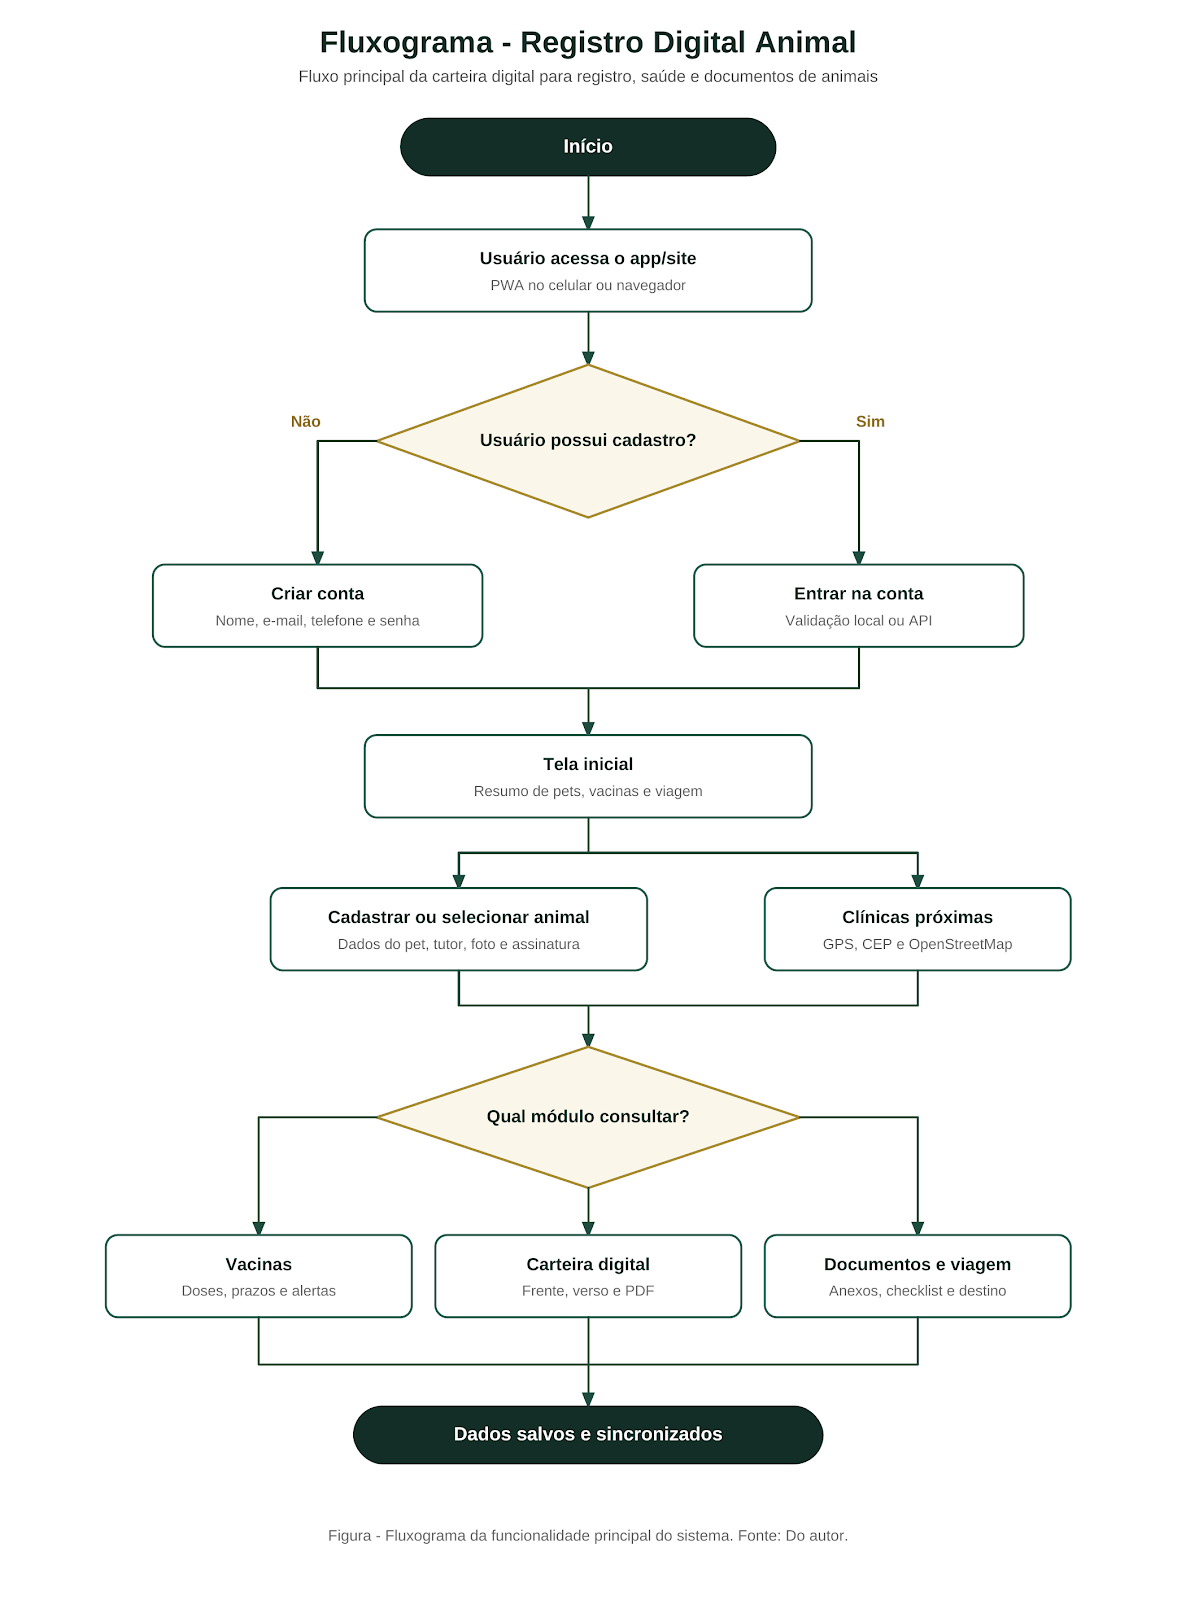
\includegraphics[scale=0.2]{Figs/fluxograma-registro-digital-animal.png}

\vspace{-0.2cm}
\begin{minipage}{\textwidth}
\footnotesize\raggedright Fonte: Elaborado pelo autor com auxílio do Codex GPT-5.5 (2026).
\end{minipage}
\end{figure}

A Figura~\ref{fig:arquitetura_tecnologias_sistema} apresenta as tecnologias por camada. No \textit{frontend}, são usados HTML5, CSS3 e JavaScript puro, com manifesto, \textit{service worker}, \textit{cache} e armazenamento local para os recursos de PWA. O \textit{backend} é escrito em JavaScript sobre Node.js, organizado como API REST, com NPM no gerenciamento das dependências. A persistência usa PostgreSQL 18, com conexão parametrizada por variáveis de ambiente. A infraestrutura da etapa de avaliação utilizou Render Postgres e Render Web Service, e o projeto também contém configuração para publicação na Vercel e execução local. A coleta complementar de novembro utilizou PostgreSQL pela integração Prisma Postgres da Vercel, distinguindo-se da infraestrutura inicial. A indisponibilidade posterior do banco hospedado limitou a recuperação de parte dos retornos da pesquisa de campo, como descrito adiante.

\begin{figure}[htbp]
\captionsetup{justification=raggedright,singlelinecheck=false,format=hang}
\caption{Arquitetura e tecnologias utilizadas no sistema Registro Digital Animal}
\label{fig:arquitetura_tecnologias_sistema}
\centering
\vspace{-0.2cm}
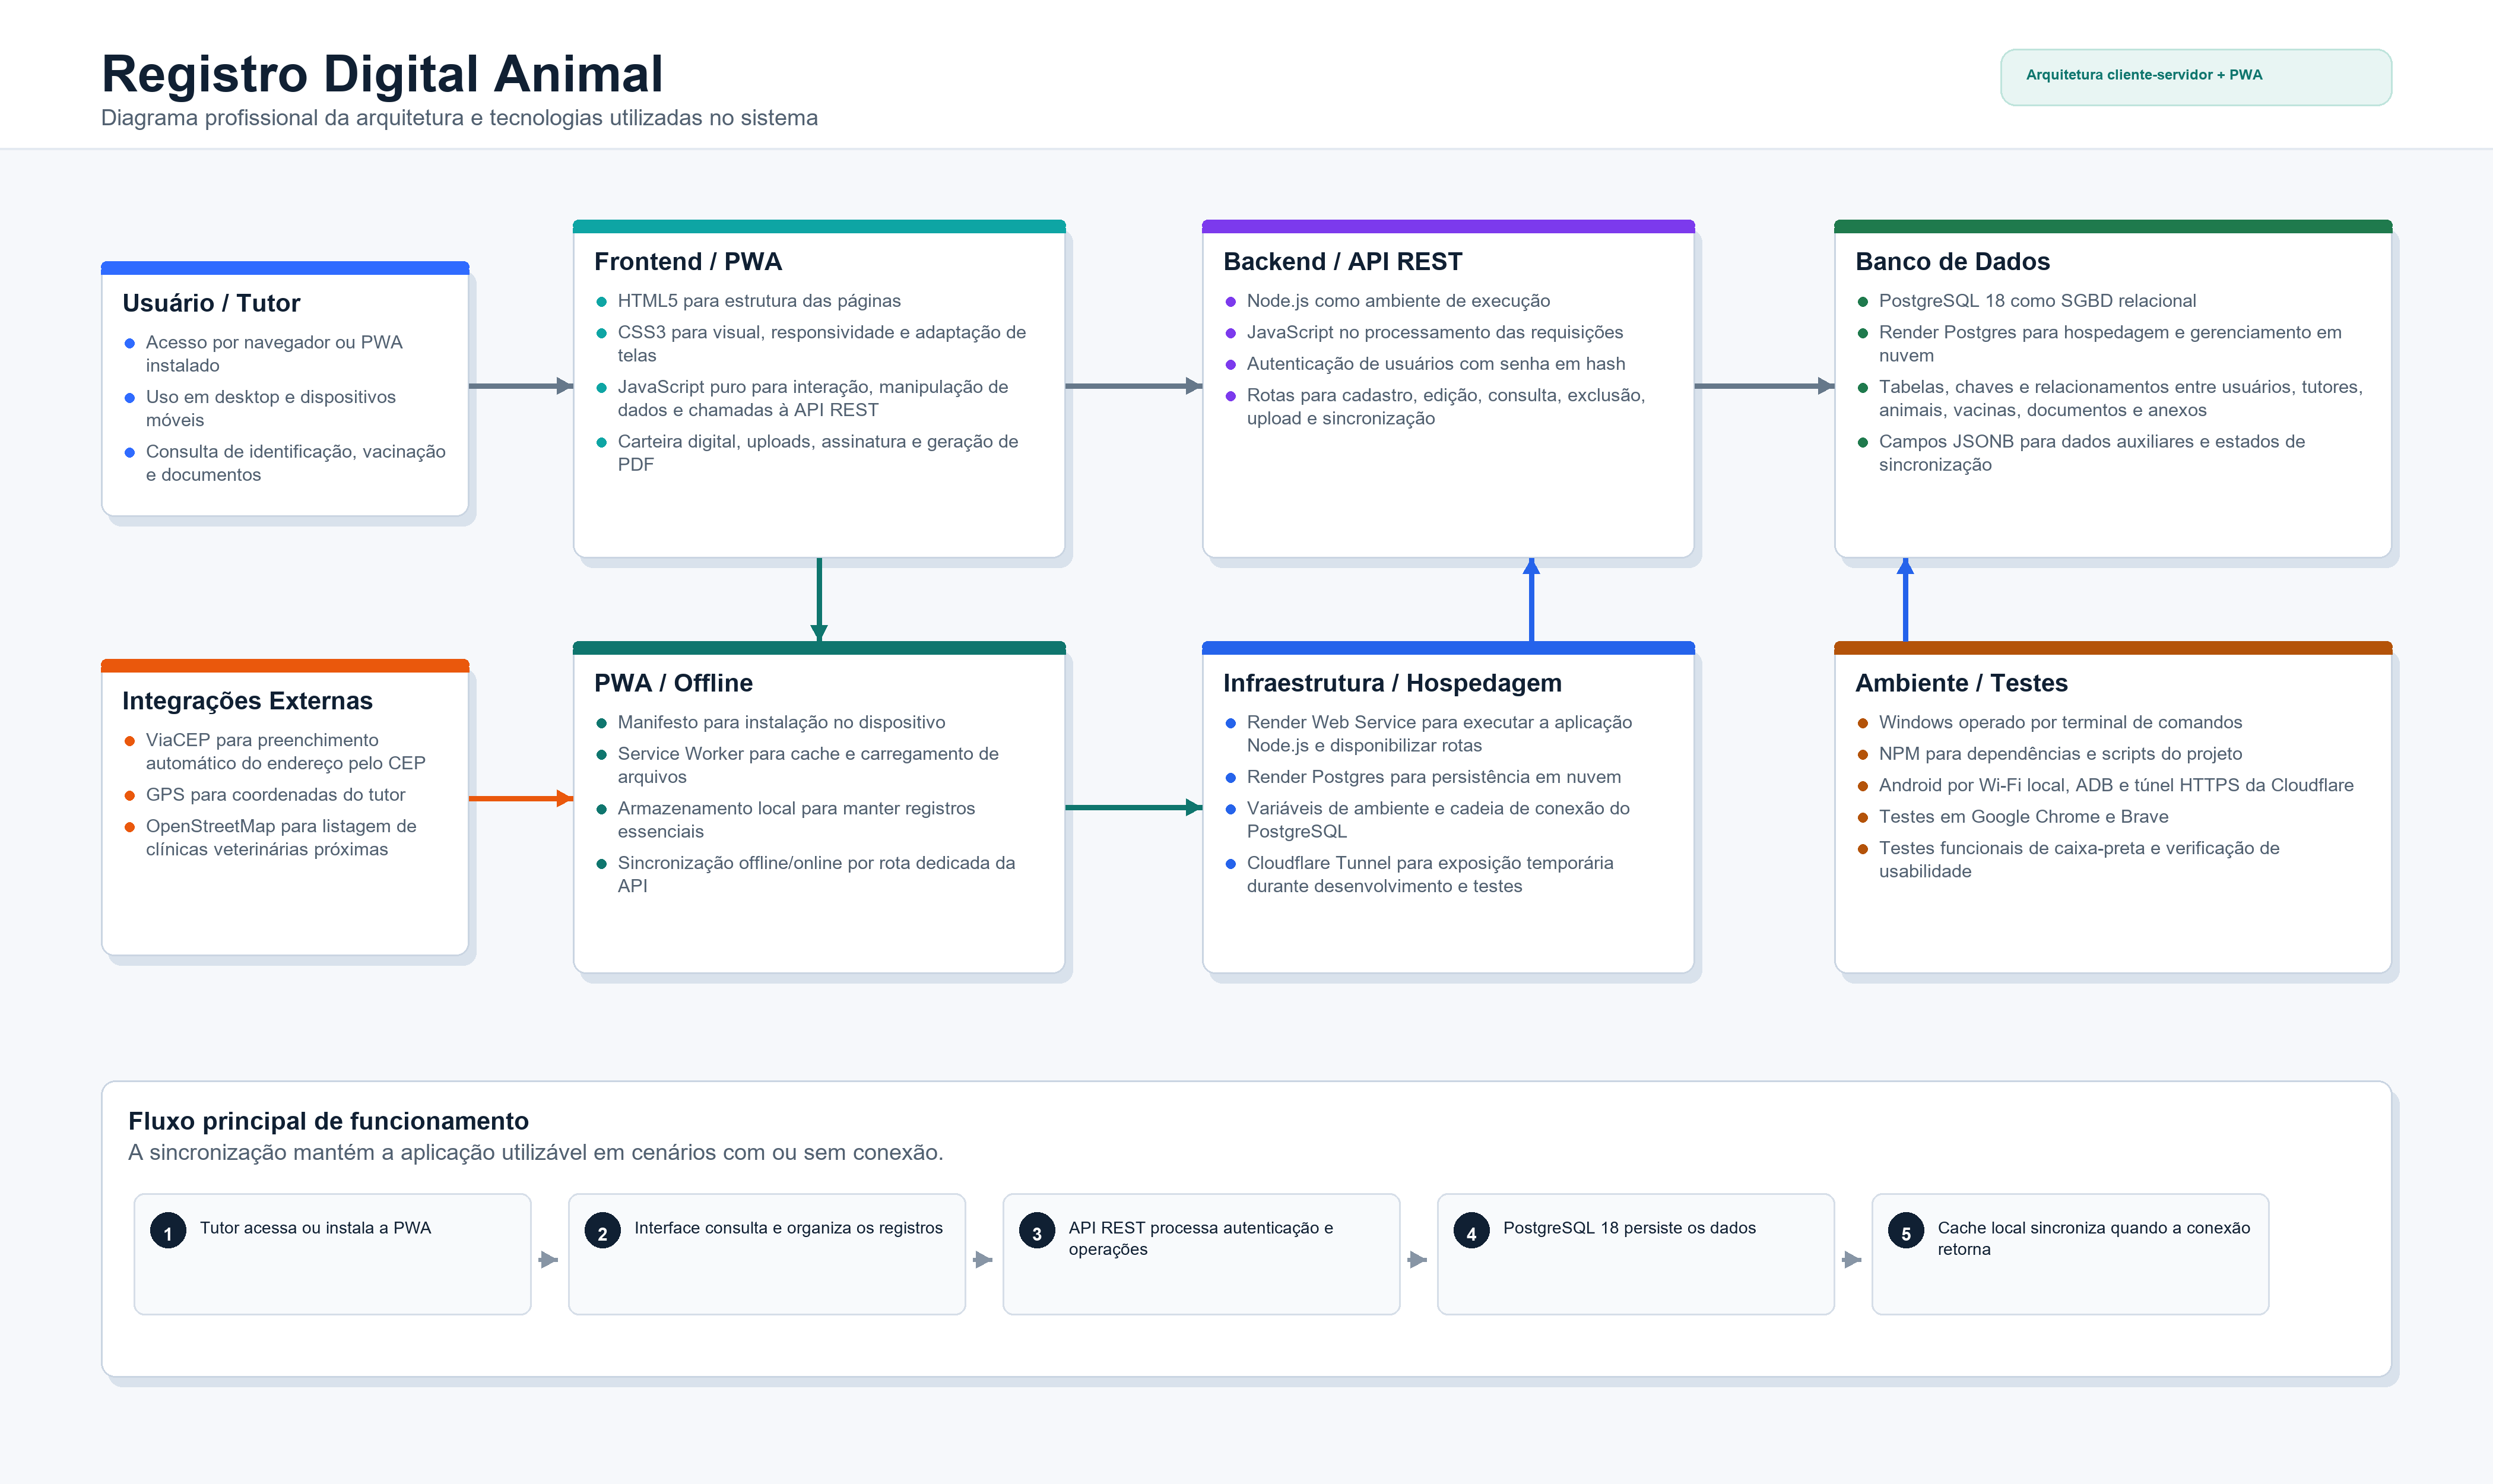
\includegraphics[width=\textwidth]{Figs/Registro_Digital_Animal_Diagrama.png}

\vspace{-0.2cm}
\begin{minipage}{\textwidth}
\footnotesize\raggedright Fonte: Elaborado pelo autor.
\end{minipage}
\end{figure}

As integrações externas incluem a API ViaCEP, para preenchimento automático de endereços, e os recursos de GPS e OpenStreetMap, para localizar clínicas veterinárias próximas ao tutor. No desenvolvimento e nos testes, foram usados Windows, os navegadores Google Chrome e Brave, dispositivos Android, rede local Wi-Fi, \textit{Android Debug Bridge} (ADB) e túnel HTTPS da Cloudflare.

A aplicação é composta por módulos de gerenciamento das informações do tutor e do animal. O módulo de usuários permite cadastro e autenticação via API, com senhas armazenadas em formato de \textit{hash}. O módulo de animais registra e edita os dados de identificação, incluindo o \textit{upload} de foto e o preenchimento automático do endereço a partir do CEP consultado na API ViaCEP, permanecendo sob responsabilidade do usuário o preenchimento do número e do complemento.

O sistema conta ainda com uma carteira digital do animal visualizável em formato frente e verso, recursos para captura de assinatura digital diretamente na aplicação, \textit{upload} de documentos do pet em imagem ou PDF e geração ou \textit{download} da carteira e de seus anexos compilados em PDF. Para auxiliar em situações de emergência e localização, a aplicação integra a geolocalização por GPS do tutor e os dados do OpenStreetMap para listar clínicas veterinárias próximas.

\subsubsection{Banco de Dados}

A Figura~\ref{fig:diagrama_banco_dados} apresenta um recorte de seis tabelas do núcleo cadastral da aplicação. A implementação contém ainda estruturas auxiliares para itens de viagem, avaliações, estado sincronizado, anexos, sincronizações em partes e eventos de uso, de modo que o diagrama não representa a totalidade do esquema. As seis estruturas representadas são:

\begin{itemize}
    \item \textbf{\texttt{pet\_app\_users}}: informações de cadastro e autenticação, incluindo nome, e-mail, telefone e \textit{hash} da senha;
    \item \textbf{\texttt{pet\_owners}}: dados do tutor vinculados ao usuário, como CPF, endereço, coordenadas de localização e contato de emergência;
    \item \textbf{\texttt{pet\_pets}}: identificação do animal, como espécie, raça, sexo, nascimento, peso, microchip, temperamento e alergias;
    \item \textbf{\texttt{pet\_vaccines}}: nome da vacina, dose, data de aplicação, data prevista da próxima dose, clínica, veterinário e lote;
    \item \textbf{\texttt{pet\_documents}}: título, categoria, data, validade e dados do anexo de cada documento;
    \item \textbf{\texttt{pet\_travel\_plans}}: destino, data da viagem, meio de transporte e animal selecionado.
\end{itemize}

\begin{figure}[htbp]
\captionsetup{
    justification=raggedright,
    singlelinecheck=false,
    format=hang
}
\caption{Recorte do núcleo cadastral do banco PostgreSQL da aplicação Registro Digital Animal}
\label{fig:diagrama_banco_dados}

\centering
\vspace{-0.2cm}

\adjustbox{
    Clip=0pt 0pt {.38\width} 0pt,
    width=.62\textwidth
}{
    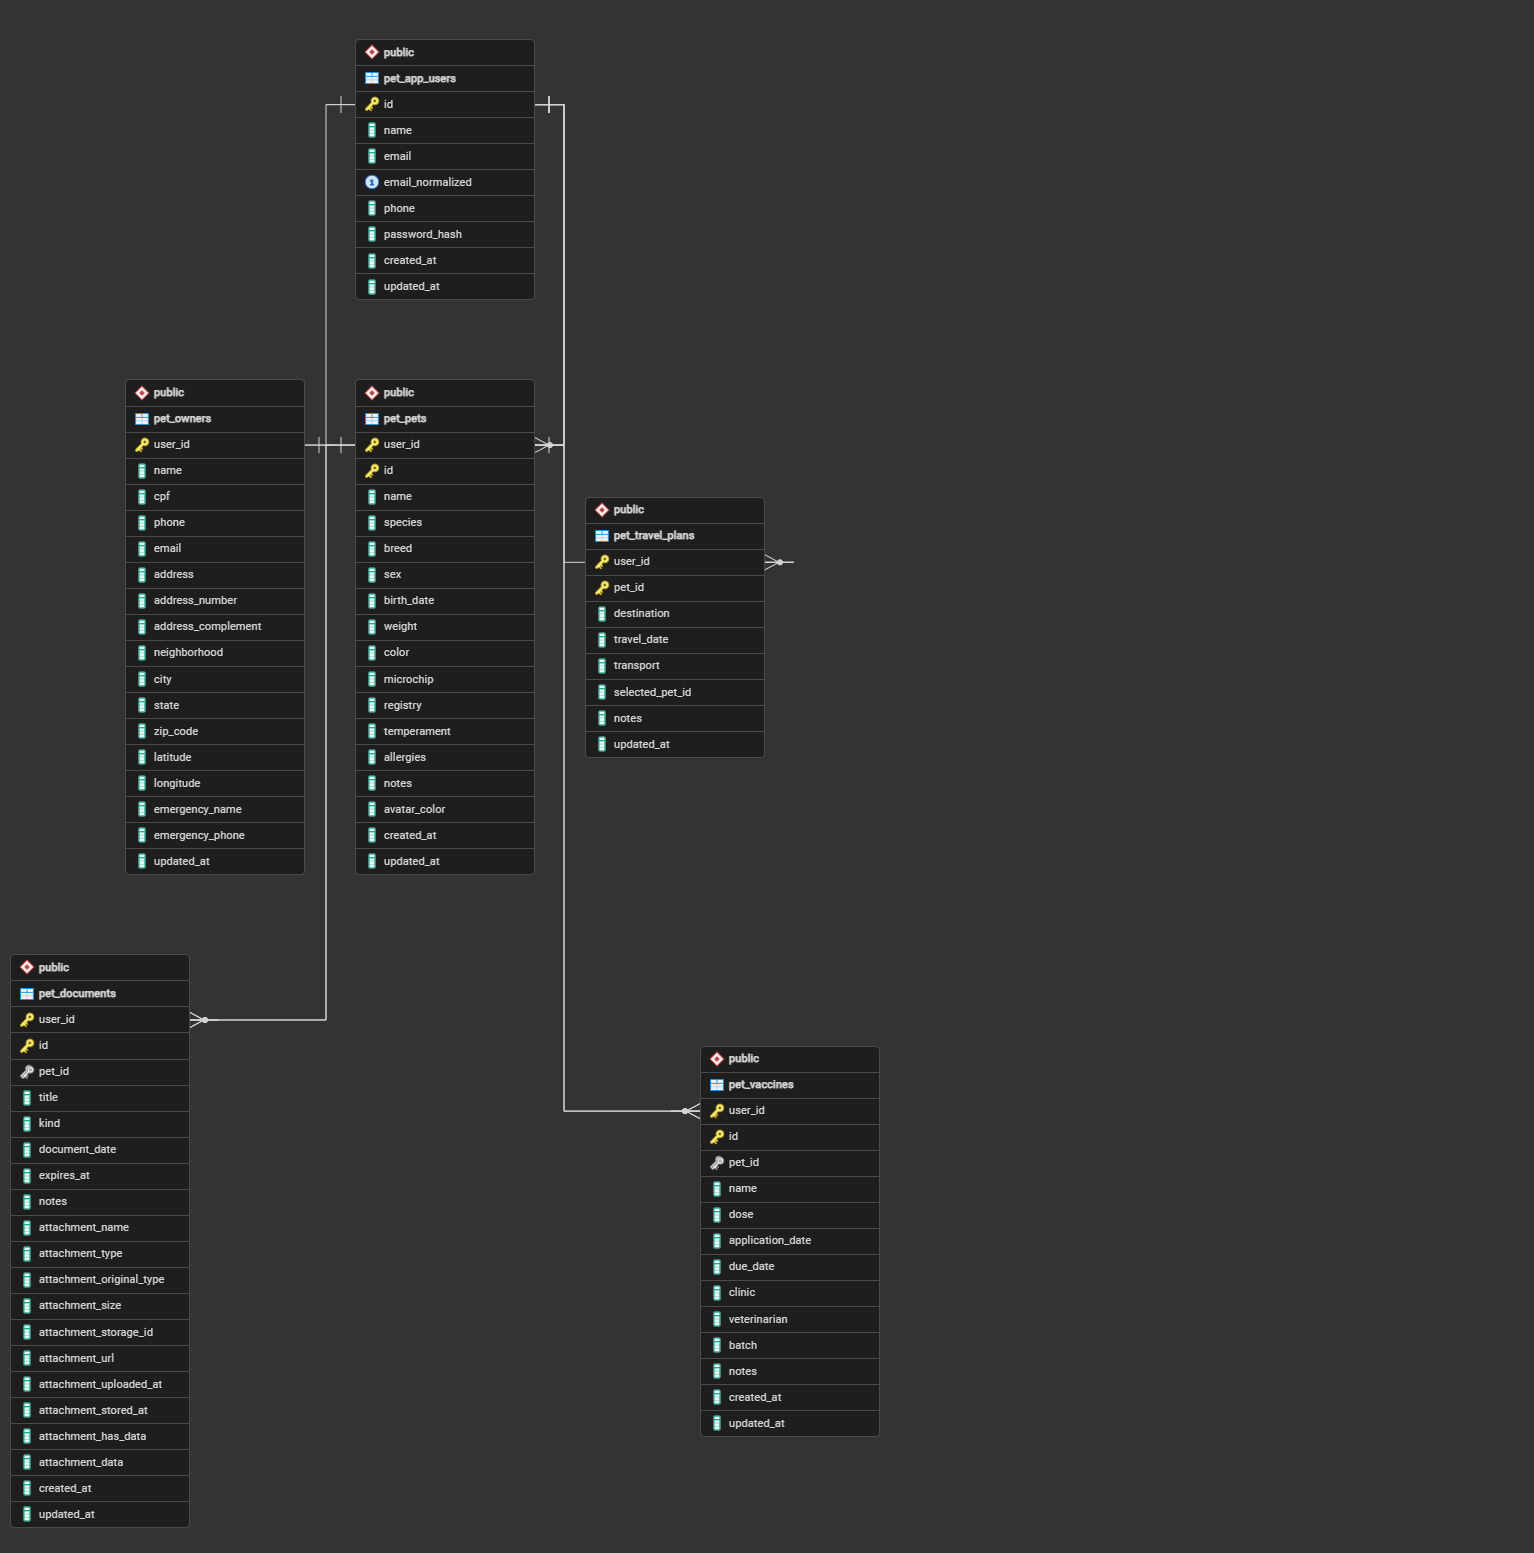
\includegraphics{Figs/Untitled.png}
}

\vspace{-0.2cm}
\begin{minipage}{\textwidth}
\footnotesize\raggedright
Fonte: Elaborado pelo autor.
\end{minipage}
\end{figure}

\subsection{Metodologia de Avaliação}

A avaliação compreendeu a verificação funcional de caixa-preta e a análise exploratória de retornos do setor veterinário. A verificação funcional comparou ações e resultados esperados; as observações sobre clareza das telas e navegação foram descritivas e não constituíram avaliação padronizada de usabilidade. A análise de retornos examinou utilidades percebidas e dificuldades relatadas, sem estimar aceitação populacional.

\subsubsection{Procedimento e cenários dos testes}

Os testes foram executados em computadores com Windows, nos navegadores Chrome e Brave, e em dispositivos Android, com acesso móvel por Wi-Fi local, depuração USB com ADB e túnel HTTPS da Cloudflare. Para cada cenário, comparou-se o comportamento observado ao esperado; a classificação \textit{Passou} correspondeu à execução da tarefa prevista e à manutenção dos dados envolvidos.

O conjunto foi organizado em 15 cenários (F01 a F15), com resultados na Tabela~\ref{tab:testes_funcionais}. Agrupados por tema, eles foram:

\begin{itemize}
    \item \textbf{F01 e F02 -- Cadastro e autenticação}: realizar o cadastro, verificar a persistência dos dados e o armazenamento da senha em \textit{hash}, efetuar o acesso e verificar a sessão e a restrição de acesso às rotas protegidas;
    \item \textbf{F03 a F05 -- Gestão do animal}: cadastrar e editar o animal com foto, informar um CEP válido e conferir o preenchimento automático do endereço, e capturar e salvar a assinatura verificando sua legibilidade e associação ao cadastro;
    \item \textbf{F06 a F08 -- Carteira e documentos}: consultar a carteira alternando entre frente e verso, enviar documentos em imagem ou PDF verificando a vinculação ao animal, e gerar o PDF conferindo dados cadastrais, vacinas, anexos e assinatura;
    \item \textbf{F09 a F12 -- Geolocalização e acesso}: obter coordenadas por GPS em Android, consultar clínicas no OpenStreetMap, navegar pelos principais fluxos em Chrome e Brave e comparar o acesso em Android por Wi-Fi, ADB e túnel Cloudflare;
    \item \textbf{F13 a F15 -- Offline e sincronização}: verificar o armazenamento e o carregamento dos recursos pelo \textit{Service Worker}, interromper a conectividade e consultar carteira e vacinas já armazenadas, e realizar alterações locais sem conexão, restabelecê-la e conferir o envio à API e a persistência no PostgreSQL.
\end{itemize} Os registros não constituem bateria exaustiva de casos negativos, concorrência ou indisponibilidade de serviços, nem documentam tempos, número de tentativas ou avaliações independentes de usabilidade.

A escala de severidade de Nielsen classifica problemas de usabilidade por frequência, impacto e persistência \cite{nielsen1994}. Como não foi preservado um protocolo de julgamento independente desses fatores por cenário, não foram atribuídas notas de severidade, e a aprovação funcional foi mantida separada dos problemas relatados pelos participantes.

\subsubsection{Procedimento da pesquisa de campo}

O convite foi dirigido a clínicas, estabelecimentos e profissionais do setor animal, identificados pelo Google Maps em Criciúma e pela plataforma Casa dos Dados para outros municípios, em seleção não probabilística. A planilha de acompanhamento registrou 96 contatos, com convites entre 11 e 18 de setembro de 2026; predominaram localidades de Santa Catarina, mas um contato era de Fortaleza, e por isso o conjunto não foi tratado como exclusivamente catarinense. O contato ocorreu pelo WhatsApp, com apresentação do pesquisador; aos que aceitaram, foram enviados o endereço do aplicativo e um vídeo de orientação, solicitando opinião sobre a experiência de uso, informações ausentes e melhorias.

Os 96 contatos resultaram em 13 aceites, 80 sem resposta e três sem interesse. Aceitar o convite, receber o material, cadastrar-se e enviar uma avaliação foram tratados como eventos distintos. A planilha indicou dois feedbacks recebidos (21 de setembro e 7 de outubro de 2026); entre os demais aceites, dez ficaram pendentes e um registrou cadastro sem avaliação. O pesquisador informou ainda um terceiro retorno, armazenado no banco do Render e indisponível após a interrupção do serviço; ele não constava como recebido na planilha, e seu conteúdo não foi analisado. O corpus inicial foi composto pelos dois retornos preservados, identificados como R1 (avaliação estruturada salva pela aplicação, com notas e comentários) e R2 (relato textual livre de uma participante, que informou ter cadastrado seus animais), sem divulgação de nomes ou estabelecimentos.

No formulário, os campos gerais registraram satisfação com as informações da carteira e avaliação do aplicativo; os itens de concordância trataram da necessidade de melhoria e da utilidade de aprimoramentos em carteira, vacinação e viagens, sem serem interpretados como satisfação. Os comentários foram agrupados por conteúdo (organização e identificação; informação vacinal; viagens; localização de clínicas; atuação veterinária) e associados a R1 ou R2. Para esses dois retornos anteriores não foram produzidas estimativas estatísticas, e a categorização, feita por um único analista, não passou por concordância entre avaliadores.

Em 4 de novembro de 2026, foi realizada uma extração complementar das tabelas de avaliações e respostas da aplicação na Vercel. A unidade de análise foi definida como o último envio válido por conta, preservando a base original e evitando contar reenvios como novas avaliações. Os itens de concordância de 1 a 5 foram apresentados individualmente, acompanhados de medianas e médias exclusivamente descritivas; zeros nos campos gerais foram tratados como respostas ausentes, por estarem fora da escala. As contas dessa extração não foram vinculadas nominalmente aos convites anteriores. A análise manteve os dois conjuntos separados, categorizou os comentários por conteúdo e relacionou as solicitações às alterações do aplicativo. Não houve nova avaliação por participantes depois dessas alterações.

\section{RESULTADOS E DISCUSSÃO}

Esta seção apresenta os resultados funcionais, a análise dos dois retornos anteriores preservados e a coleta complementar de novembro. Cada fonte foi discutida conforme seu alcance: tarefas dos cenários definidos, relatos individuais, respostas estruturadas por conta e alterações técnicas posteriores. Os conjuntos não foram agregados como uma única amostra de participantes.

\subsection{Resultados dos cenários funcionais}

A Tabela~\ref{tab:testes_funcionais} apresenta os resultados dos 15 cenários. A classificação expressa o resultado funcional registrado, sem equivalência com medida de usabilidade.

\begin{table}[htbp]
\centering
\caption{Resultados registrados para os cenários funcionais do sistema}
\label{tab:testes_funcionais}
\par\vspace{4pt}
\small
\setlength{\tabcolsep}{4pt}
\renewcommand{\arraystretch}{1.1}
\begin{tabular}{@{}p{0.08\linewidth} p{\dimexpr0.76\linewidth-4\tabcolsep\relax} p{0.16\linewidth}@{}}
\hline
\textbf{ID} & \textbf{Cenário de teste avaliado} & \textbf{Resultado} \\
\hline
F01 & Cadastro de usuário e armazenamento de senha com \textit{hash} & Passou \\
F02 & Autenticação do usuário e controle de sessão na API REST & Passou \\
F03 & Cadastro e edição de perfil de animal com \textit{upload} de foto & Passou \\
F04 & Preenchimento automático de endereço via API ViaCEP a partir do CEP & Passou \\
F05 & Captura e salvamento de assinatura digital no formulário & Passou \\
F06 & Visualização interativa da carteira digital, com frente e verso & Passou \\
F07 & \textit{Upload} e vinculação de documentos clínicos em imagem ou PDF & Passou \\
F08 & Geração e exportação da carteira digital consolidada em PDF & Passou \\
F09 & Captura de coordenadas de geolocalização via GPS móvel & Passou \\
F10 & Consulta de clínicas veterinárias próximas via OpenStreetMap & Passou \\
F11 & Responsividade e navegação em \textit{desktop} nos navegadores Chrome e Brave & Passou \\
F12 & Acesso móvel em Android via Wi-Fi, ADB e túnel Cloudflare & Passou \\
F13 & Armazenamento e execução de \textit{cache} pelo \textit{Service Worker} & Passou \\
F14 & Acesso e consulta offline aos dados da carteira e das vacinas & Passou \\
F15 & Sincronização offline-online de registros no banco PostgreSQL & Passou \\
\hline
\end{tabular}
\par\vspace{2pt}
{\footnotesize\raggedright Fonte: Elaborado pelo autor.\par}
\end{table}

Os 15 cenários foram registrados como aprovados nas condições descritas. O resultado se restringe às tarefas previstas: não caracteriza ausência de falhas em outros cenários, não substitui avaliação de usabilidade com usuários e não permite estimar confiabilidade em produção.

Nos cenários de autenticação (F01 e F02), a API realiza o cadastro com senhas em \textit{hash} e restringe o acesso às rotas protegidas. Nos de gestão do animal (F03 a F05), o formulário se comporta de forma consistente, a integração com o ViaCEP reduz o preenchimento manual de logradouro, bairro, cidade e estado, e a assinatura mantém a legibilidade e a associação ao cadastro. Nos de carteira e documentos (F06 a F08), a aplicação permite a visualização organizada dos dados, a alternância entre frente e verso, o envio de documentos e a exportação consolidada em PDF com dados cadastrais, vacinas, anexos e assinatura, o que reforça a proposta de alternativa digital à caderneta física.

Os testes de mobilidade e geolocalização (F09 a F12) mostraram comportamento estável nas diferentes formas de acesso, com listagem de estabelecimentos veterinários próximos em Android e funcionamento equivalente por Wi-Fi, ADB e túnel Cloudflare. Por fim, os cenários F13 a F15 validaram o funcionamento offline e a sincronização: o \textit{Service Worker} e o \textit{cache} mantêm a aplicação acessível sem internet, com consulta aos dados essenciais da carteira e das vacinas já salvos, e os registros pendentes são enviados à API e persistidos no PostgreSQL quando a conectividade volta.

\subsection{Análise dos retornos anteriores preservados da pesquisa de campo}

No acompanhamento inicial, o registro de recrutamento apresentou 13 aceites entre 96 contatos (13,5\%), e somente dois tiveram feedback marcado como recebido. Esses números descrevem o acompanhamento dos convites e não medem satisfação ou utilização efetiva. A Tabela~\ref{tab:recrutamento} resume as etapas documentadas.

\begin{table}[htbp]
\centering
\caption{Situação dos contatos e dos retornos no acompanhamento inicial}
\label{tab:recrutamento}
\small
\setlength{\tabcolsep}{5pt}
\renewcommand{\arraystretch}{1.1}
\begin{tabular}{@{}p{\dimexpr0.84\linewidth-2\tabcolsep\relax} r@{}}
\hline
\textbf{Etapa ou situação registrada} & \textbf{Quantidade} \\
\hline
Contatos com convite registrado & 96 \\
Aceitaram participar & 13 \\
Sem resposta ao convite & 80 \\
Não interessados & 3 \\
Aceites com feedback marcado como recebido & 2 \\
Aceites com feedback pendente & 10 \\
Aceite com cadastro, sem feedback, conforme observação & 1 \\
Retornos preservados incluídos na análise & 2 \\
Retorno adicional informado, indisponível e excluído & 1 \\
\hline
\end{tabular}
\par\vspace{2pt}
{\footnotesize\raggedright Fonte: Elaborado pelo autor.\par}
\end{table}

A Tabela~\ref{tab:resumo_qualitativo} relaciona os aspectos analisados aos registros que os sustentam. As descrições são menções individuais, sem indicação de prevalência entre profissionais veterinários.

\begin{table}[htbp]
\centering
\caption{Síntese dos comentários presentes nos dois retornos preservados}
\label{tab:resumo_qualitativo}
\small
\setlength{\tabcolsep}{4pt}
\renewcommand{\arraystretch}{1.1}
\begin{tabular}{@{}p{0.24\linewidth} p{\dimexpr0.66\linewidth-4\tabcolsep\relax} p{0.10\linewidth}@{}}
\hline
\textbf{Aspecto} & \textbf{Comentário ou sugestão registrada} & \textbf{Fonte} \\
\hline
Identificação e preenchimento & Dificuldade para informar o peso de 16,3; valorização de informações mais detalhadas sobre o animal. & R1 \\
Registro de vacinas & Questionamento sobre a necessidade do campo de quantidade de aplicação, considerado assunto de análise veterinária. & R1 \\
Organização e consulta & Utilidade dos dados para preenchimento pelo tutor e comunicação das informações durante o atendimento; navegação descrita como fácil. & R2 \\
Identificação por microchip & Valorização do registro de microchip como informação útil em situações de resgate. & R2 \\
Planejamento de viagens & Área descrita como completa e útil para organização antecipada de documentos. & R2 \\
Localização de clínicas & Utilidade da busca de estabelecimentos próximos e sugestão de destacar os que atendem 24 horas. & R2 \\
Atuação veterinária & Sugestão de área profissional com identificação pelo registro de conselho, consulta por microchip e registros de atendimento. & R2 \\
\hline
\end{tabular}
\par\vspace{2pt}
{\footnotesize\raggedright Fonte: Elaborado pelo autor a partir dos retornos preservados.\par}
\end{table}

Em R1, os campos gerais apresentaram nota 5 para as informações da carteira e nota 4 para a avaliação do aplicativo, em escala de 1 a 5; por pertencerem a um único retorno, não foram tratadas como média de satisfação. A dificuldade com peso decimal apareceu no exemplo de um animal com 16,3, registrado como 16 porque o valor exato não foi aceito na interação descrita. O achado evidencia uma limitação percebida no preenchimento, sem permitir atribuir sua causa ao navegador, à versão do aplicativo ou à validação de um campo específico. O comentário sobre a quantidade de aplicação indica a necessidade de revisar a clareza e a pertinência dos dados do módulo de vacinação, considerando a distinção entre registro pelo tutor e avaliação profissional.

R2 destacou a organização das informações e a facilidade de localizá-las, e considerou úteis os dados de identificação, o registro de microchip, o planejamento de viagens e a busca de clínicas próximas. A sugestão de destacar estabelecimentos 24 horas indica que a proximidade, isoladamente, pode ser insuficiente em situação de urgência, sem comprovação de redução do tempo de atendimento ou melhoria de desfechos clínicos. A sugestão de uma área veterinária, com consulta por microchip e registros de atendimento, amplia o problema para o compartilhamento de informações entre tutores e profissionais e exigiria investigar responsabilidades, autorização de acesso e verificação de identidade profissional; a menção a um número de conselho, por si só, não demonstra mecanismo suficiente de validação. Foi mantida como possibilidade de investigação, e não como funcionalidade entregue. Nesses dois retornos anteriores, não foram identificados comentários que comprovem aceitação do funcionamento offline, da exportação em PDF ou de notificações de revacinação; esses recursos foram descritos na avaliação técnica, e sua apreciação pelos participantes não foi presumida.

\subsection{Avaliações estruturadas registradas em novembro de 2026}
\label{sec:feedbacks_novembro}

Uma coleta complementar foi consultada em 4 de novembro de 2026 no PostgreSQL disponibilizado pela integração Prisma Postgres da Vercel. A consulta relacionou a tabela principal de avaliações às respostas de cada pergunta pela chave composta de usuário e avaliação. Foram encontrados cinco envios vinculados a quatro contas. Dois envios pertenciam à mesma conta, apresentavam notas e comentários idênticos e foram registrados com aproximadamente 15 segundos de diferença. Para evitar a contagem duplicada, foi mantido na análise apenas o envio mais recente dessa conta; nenhum registro foi excluído do banco. O recorte resultou em quatro avaliações, uma por conta, identificadas como N1 a N4 pela ordem cronológica dos envios selecionados, totalizando 24 respostas válidas às seis afirmações de concordância.

Conta distinta não comprova participante distinto ou independência entre respostas. A extração não estabeleceu profissão, município, experiência de uso ou vínculo dessas contas com os 13 aceites da planilha de recrutamento. Por isso, os novos registros não foram somados aos dois retornos anteriores para anunciar seis participantes, nem utilizados para recalcular a taxa de resposta dos convites de setembro. A caracterização se restringe às avaliações registradas na aplicação. Os nomes, endereços eletrônicos e identificadores técnicos das contas foram omitidos da apresentação dos resultados.

Os registros selecionados ocorreram em 4 de novembro de 2026, entre 15h15 e 15h29, no horário de Brasília; o banco apresenta os horários em UTC. A proximidade temporal dos envios caracteriza o momento de registro e não demonstra duração dos testes, tempo de uso do aplicativo ou exposição equivalente às funcionalidades. A seleção do último envio por conta é uma regra de preparação do corpus e não uma comprovação da identidade de quem respondeu.

\subsubsection{Escalas e tratamento das respostas}

O formulário contém dois campos gerais de avaliação e seis afirmações distribuídas entre necessidade de melhoria e utilidade de sugestões. A escala de concordância varia de 1 (discordo totalmente) a 5 (concordo totalmente), com 2 para discordância parcial, 3 para posição neutra e 4 para concordância parcial. As duas partes têm sentidos diferentes: discordar de que uma área precisa melhorar representa baixa concordância com o problema enunciado, enquanto concordar com uma sugestão representa utilidade percebida para uma possível mudança. Consequentemente, os seis itens não foram somados em um índice geral de satisfação ou de usabilidade.

Nos campos gerais, N1 e N2 registraram nota 5 tanto para satisfação com as informações da carteira quanto para avaliação do aplicativo, e N4 atribuiu nota 4 aos dois campos. N3 apresentou zero em ambos. Como zero não integra a escala de 1 a 5 apresentada ao usuário, foi tratado como ausência de resposta válida nesses campos, sem eliminar as seis respostas de concordância válidas dessa avaliação. Para cada campo geral, portanto, houve três respostas válidas: duas notas 5 e uma nota 4, com média descritiva de 4,67 e mediana 5. Esses números descrevem somente os registros disponíveis e não estimam satisfação populacional.

\begin{table}[htbp]
\centering
\caption{Respostas às afirmações de concordância, após seleção por conta}
\label{tab:likert_novembro}
\small
\setlength{\tabcolsep}{4pt}
\renewcommand{\arraystretch}{1.15}
\begin{tabular}{@{}p{\dimexpr0.53\linewidth-8\tabcolsep\relax}rrrrrr@{}}
\hline
\textbf{Afirmação resumida} & \textbf{N1} & \textbf{N2} & \textbf{N3} & \textbf{N4} & \textbf{Média} & \textbf{Med.} \\
\hline
Carteirinha precisa de informações mais claras e completas & 1 & 2 & 2 & 4 & 2,25 & 2 \\
Vacinas precisam apresentar melhor datas, clínica e situação & 1 & 2 & 2 & 2 & 1,75 & 2 \\
Viagens precisam organizar melhor checklist e documentos & 1 & 1 & 1 & 1 & 1,00 & 1 \\
Mais campos opcionais na carteirinha ajudariam na identificação & 2 & 2 & 4 & 4 & 3,00 & 3 \\
Alertas, filtros e destaque para vacinas atrasadas seriam úteis & 1 & 4 & 5 & 5 & 3,75 & 4,5 \\
Checklist por pet com dados e lembretes ajudaria no planejamento & 1 & 4 & 5 & 5 & 3,75 & 4,5 \\
\hline
\end{tabular}
\par\vspace{2pt}
{\footnotesize\raggedright Fonte: Elaborado pelo autor a partir das avaliações consultadas em 4 de novembro de 2026. Cada linha possui quatro respostas. Médias são sínteses descritivas de itens ordinais, acompanhadas das respostas individuais e medianas.\par}
\end{table}

A Tabela~\ref{tab:likert_novembro} mostra discordância total dos quatro registros quanto à afirmação de que a organização de viagens precisava melhorar. Isso não significa rejeição a novas funcionalidades: na afirmação sobre utilidade de checklist por pet, três contas concordaram parcial ou totalmente e uma discordou totalmente. O mesmo padrão apareceu no item sobre alertas de vacinas, com notas 4, 5 e 5 nos registros favoráveis e nota 1 no restante. A concordância com incrementos pode coexistir com baixa concordância com uma deficiência geral da tela atual. Para os campos opcionais da carteira, as respostas se dividiram entre duas discordâncias parciais e duas concordâncias parciais, sem posição uniforme.

Não foram realizados testes de significância, inferência populacional ou avaliação psicométrica do instrumento. A distribuição individual e as medianas ajudam a explicitar a heterogeneidade do pequeno conjunto. Também não se atribuiu nota de severidade de Nielsen a partir das notas de concordância: opinião sobre uma melhoria e severidade observada de um problema são medidas distintas.

\subsubsection{Comentários e transformação em requisitos}

N1 não acrescentou comentários textuais. N2 sugeriu uma área de notificações para alertar sobre vencimentos e valorizou a organização antecipada de uma futura viagem. N3 pediu que fossem apresentadas todas as vacinas vencidas, e não apenas uma; nos outros comentários, informou não ter sugestões naquele momento. N4 solicitou um resumo mais informativo das vacinas vencidas, exemplificando a apresentação de dois nomes e da quantidade restante. Também considerou úteis os alertas e sugeriu selecionar vários pets para uma viagem, escolher entre checklist geral ou separado e acrescentar itens relacionados a necessidades específicas.

Os comentários foram categorizados por seu conteúdo, preservando o significado mesmo quando preenchidos em campo associado a outro assunto. Por exemplo, a solicitação de mostrar todas as vacinas vencidas foi registrada em um comentário da seção sobre carteirinha, mas descreve um requisito de apresentação da informação vacinal. Essa distinção evita interpretar o nome do campo como substituto da leitura do relato.

A priorização considerou especificidade do pedido e relação com as tarefas já implementadas. As solicitações resultaram em três frentes: visibilidade dos prazos, síntese das pendências e flexibilidade do planejamento de viagens. Não se concluiu que todos os usuários necessitariam das mesmas funções. A Tabela~\ref{tab:rastreabilidade_feedbacks} relaciona as manifestações às alterações realizadas na revisão do aplicativo.

\begin{table}[htbp]
\centering
\caption{Rastreabilidade entre comentários e alterações do aplicativo}
\label{tab:rastreabilidade_feedbacks}
\small
\setlength{\tabcolsep}{4pt}
\renewcommand{\arraystretch}{1.15}
\begin{tabular}{@{}p{\dimexpr0.28\linewidth-2\tabcolsep\relax}p{\dimexpr0.62\linewidth-2\tabcolsep\relax}p{0.10\linewidth}@{}}
\hline
\textbf{Necessidade relatada} & \textbf{Alteração implementada} & \textbf{Fonte} \\
\hline
Lembrar vencimentos & Central de avisos de vacinas e documentos, com vencidos, próximos 30 dias, filtros por categoria e acesso ao registro. & N2, N4 \\
Mostrar todas as vacinas vencidas & Listagem individual das pendências e síntese na carteira com quantidade, dois nomes e indicação das demais; ausência de registros não aparece como situação em dia. & N3, N4 \\
Preparar futuras viagens & Documentos do pet reunidos na tela de viagem e avisos de viagens nos próximos 30 dias com checklist pendente. & N2 \\
Organizar vários pets & Seleção de acompanhantes no plano de viagem, com escolha entre listas individuais e checklist compartilhado para o grupo selecionado. & N4 \\
Contemplar necessidades específicas & Inclusão e remoção de itens adicionais do checklist e campo de anotações; marcações compartilhadas se propagam somente ao grupo. & N4 \\
\hline
\end{tabular}
\par\vspace{2pt}
{\footnotesize\raggedright Fonte: Elaborado pelo autor. As alterações representam resposta de desenvolvimento aos comentários, sem comprovação de melhora de usabilidade após a mudança.\par}
\end{table}

Os avisos foram implementados no interior da aplicação e calculados com base nas datas e nos dados disponíveis no dispositivo. O prazo do dia corrente é apresentado como vencimento no dia, e registros sem data válida não são classificados como regulares. O recurso não representa envio de notificações ao sistema operacional com o aplicativo fechado. Seu alcance depende da completude dos registros, da data do dispositivo e da atualização dos dados, inclusive da sincronização quando o uso ocorre em mais de um aparelho.

A revisão foi acompanhada de seis testes automatizados, executados com dados fictícios, para regras de data, contagem de vacinas vencidas, manutenção de todas as pendências na lista, seleção de lembretes de documentos e viagens, propagação de marcações e remoções no grupo e preservação de listas após serialização em JSON. Esses testes verificam regras técnicas e não equivalem a uma nova avaliação com participantes. As melhorias posteriores à coleta não receberam notas de satisfação retrospectivas, nem foram apresentadas como responsáveis por aumento comprovado de adesão à vacinação, redução de esquecimentos ou maior facilidade de uso.


\subsection{Limitações e ameaças à validade}

A avaliação funcional se limitou aos cenários e ambientes descritos, sem cobertura exaustiva de entradas inválidas, falhas de serviços externos, conflitos entre dispositivos ou perda de conexão durante o envio de anexos. A ausência de medidas de tempo, repetição e comparação com outra solução restringe conclusões sobre desempenho e facilidade de uso, e a observação feita no contexto de desenvolvimento pode favorecer a familiaridade com os fluxos, reduzindo a identificação de dificuldades de novos usuários.

Na pesquisa de campo, a seleção por conveniência, os dois retornos anteriores, a caracterização incompleta dos respondentes, a perda de um retorno e a categorização por um único analista limitam a comparação entre participantes. Na coleta complementar, quatro contas não comprovam quatro participantes independentes, e sua correspondência com os contatos anteriores não foi estabelecida. A concentração dos envios em um mesmo dia, a repetição por uma conta e a ausência de resposta válida aos campos gerais em outra exigiram explicitar critérios de seleção e denominadores. A pequena quantidade de avaliações e a ausência de reavaliação após as alterações impedem atribuir melhoria de usabilidade às funcionalidades adicionadas. A diferença entre aceites e retornos preservados introduz viés de não resposta: as percepções disponíveis podem não representar quem não respondeu ou aceitou sem avaliar. Os resultados não demonstram redução do uso de registros físicos, aumento de adesão à vacinação ou superioridade em relação a aplicativos existentes, e a pesquisa não avaliou a autenticação de autoria da assinatura capturada nem a aceitação documental do PDF por terceiros. Essas limitações delimitam a contribuição como desenvolvimento de um artefato e avaliação exploratória de seu funcionamento e de necessidades percebidas.

\section{CONCLUSÃO}

Este trabalho abordou a organização de informações de identificação, vacinação e documentos clínicos de animais de estimação por meio da aplicação multiplataforma Registro Digital Animal. O objetivo de desenvolver e avaliar o funcionamento da solução foi atendido no âmbito dos módulos implementados e dos cenários descritos: a aplicação reúne cadastro de tutores e animais, carteira digital, registros vacinais, documentos e recursos de consulta em computadores e dispositivos móveis, incluindo acesso a dados previamente armazenados e sincronização posterior.

Os 15 cenários funcionais foram registrados como aprovados nas condições avaliadas, o que indica atendimento às tarefas previstas, mas não comprova ausência de falhas nem usabilidade generalizável. Os dois retornos preservados complementaram a avaliação técnica ao apontar utilidade na organização dos dados e no planejamento de viagens, junto com dificuldades específicas: preenchimento de peso decimal, pertinência dos campos vacinais, identificação de clínicas com atendimento 24 horas e possibilidades de participação profissional. A aprovação de fluxos funcionais não eliminou as dificuldades relatadas, o que reforça a importância de complementar testes técnicos com observação do uso.

A coleta complementar acrescentou quatro avaliações, uma por conta, após desconsideração de um envio repetido, sem comprovação de quatro novos participantes independentes. Os comentários foram convertidos em avisos internos de prazos, resumo de todas as vacinas vencidas, acesso aos documentos na área de viagens e escolha de checklist individual ou compartilhado, com itens adicionais. As regras receberam seis testes automatizados com dados fictícios. Esse ciclo documenta a resposta do desenvolvimento às necessidades relatadas, mas não constitui evidência de satisfação com a versão modificada ou de redução de esquecimentos, pois não houve reavaliação por participantes.

A contribuição prática é um artefato que reúne diferentes registros do animal em uma interface acessível ao tutor. Como contribuição ao conhecimento no contexto estudado, a avaliação exploratória mostrou a necessidade de considerar conjuntamente a disponibilidade da informação, a precisão do preenchimento e sua adequação ao uso profissional, oferecendo requisitos e questões para novas avaliações, sem afirmar generalização teórica ou superioridade da solução. O alcance dessa contribuição foi limitado pelo conjunto de testes, pela ausência de comparação com registros físicos, pelo pequeno conjunto de evidências (dois retornos anteriores preservados, quatro avaliações de contas distintas na coleta complementar e um retorno anterior indisponível) e pela seleção não probabilística, que impede estender as percepções a todos os tutores ou profissionais. A redução da dependência de documentos físicos permaneceu como benefício pretendido, sem mensuração.

Duas lições merecem registro. A primeira é que o armazenamento remoto não dispensa procedimentos de preservação dos dados de avaliação: a perda de um registro evidenciou a necessidade de cópias independentes e de documentação da coleta. A segunda é distinguir correção de uma operação, clareza da interface e utilidade percebida, dimensões que podem apresentar resultados diferentes e exigem evidências próprias.

Como trabalhos futuros, propõe-se investigar, com tutores e veterinários de perfis distintos, se a carteira digital altera o tempo de localização das informações, a completude dos registros e a frequência de consulta em comparação à documentação física, além de avaliar o acompanhamento de prazos vacinais ao longo do tempo. Também se recomenda testar cenários de conectividade intermitente, edições concorrentes e recuperação de dados, bem como estudar a participação veterinária e a busca de clínicas em urgência, considerando qualidade dos dados, autorização de acesso e confiabilidade da informação. Conclui-se que a aplicação constitui uma alternativa tecnicamente implementada para centralizar os registros no contexto delimitado, acompanhada de evidências iniciais de funcionamento e de necessidades de aprimoramento.

\bibliographystyle{abntex2-alf}
\renewcommand{\refname}{REFERÊNCIAS}
\bibliography{referencias}

\end{document}